\documentclass[12pt]{article}

\title{Research training portfolio}
\author{Wessel Stoop}

\usepackage{covington}
\usepackage{graphicx}
\usepackage{natbib}

\renewcommand{\familydefault}{\sfdefault}

\let\stdsection\section
\renewcommand\section{\newpage\stdsection}

\begin{document}
\maketitle

\begin{table}[h]
\begin{tabular}{ll}
Name&Wessel Stoop\\
Student numbers&s0808709 (Nijmegen), u1249664 (Tilburg)\\
Project&Fowlt, a context-based spelling checker\\
Supervisor&Antal van den Bosch\\
Period&September - December 2012\\
\end{tabular}
\end{table}

\section{Introduction}
Fowlt is the English version of the Dutch spelling checker Valkuil.net. Both Valkuil and Fowlt are unlike most well-known spell checkers (like the one in Microsoft Word): whereas these spelling checkers mostly try to find errors by comparing all words to a built-in dictionary and flag the word as an error if they can't find a match, Valkuil and Fowlt are 'context-based'. This entails that they also take into account the context, which is the words around every word. If, for a particular word, they expected another word based on the context, and the algorithm is really certain about it, it is flagged as an error. This means, for example, that Fowlt is able to replace the incorrect "there' in "there really nice people" into "they're" simply because "there" usually isn't followed by "really nice people", while "they're" is. 
\\\indent
To be able to make these kinds of correction suggestions, Fowlt makes use of language models. These models are created by giving lots of texts to the machine learning software TiMBL and WOPR. It's on the basis of these texts the model knows "there" mostly is not followed by "really nice people". However, this also means that if the context of a particular error is very different from what the model has seen in the training data, it won't be able to correct the error. This means users should be aware of the fact that, although Fowlt can recognize more kinds of errors than regular spell checkers, it might still miss a few. This is particularly true because Fowlt has been taught to only flag a word as an error if the algorithms are really sure about it.

\section{What I have done}
The best way to get a good overview of what I have done is probably to look at Fowlt's internal structure, so that's what I present in the next section. The first part of my internship basically consisted of adding the modules described below, one by one. To get a better idea of what parts took more time to 'get right', I also added a section about problems I encountered.

\subsection{Project structure}
Fowlt exist of multiple little spelling checkers, specialized in doing one thing. These spelling checkers are called 'modules'. Fowlt consists of four context-free modules (relatively similar to normal spelling checkers functionality) and, as I write this, sixteen context-based modules. This number will probably be different when you read this, though, as new context-based modules are created easily, and can be removed if it turns out they're not accurate enough. Although it is possible to run Fowlt as a stand-alone application, most people will use it as a web application. I will devote a subsection to this 'web shell' around Fowlt as well.

%Plaatje toevoegen

\subsubsection{The processchain}
In Fowlt's main script, fowlt\_processchain.py, all modules are started up, their outputs are collected and are all saved in xml form. Making changes in this script (based on the ones for Valkuil, written by Maarten van Gompel) to make sure the new English based modules worked correctly, is one of the main things I did during my internship. 

\subsubsection{ErrorlistChecker (context-free)}
Martin Reynaert provided us with a large list of common typos and their corrections. This module, written by me, checks for every word in the input whether it's in the errorlist, and adds the correction when it is.

\subsubsection{LexiconChecker (context-free)}
Google provided us with an enormous list of word frequencies on the internet in 2008. The LexiconChecker checks for every word in the input whether there's a word on the frequencylist that is very similar to it, but much more frequent.

\subsubsection{RunonChecker (context-free)}
The RunonChecker also uses Google's list, but uses it to check if any spaces were forgotten in the input. This is done by looking whether splitting up long words produces two words which both are much more frequent that the original word.

\subsubsection{SplitChecker (context-free)}
The SplitChecker is the exact opposite of the RunonChecker: instead of looking whether any spaces are forgotten, it checks whether any spaces have to be added. This is done by looking whether each combination of two words produces a word which is much more frequent than the two original words.

\subsubsection{WOPRChecker (context-based)}
The WOPRChecker contacts WOPR, running on a server on localhost or elsewhere. It gives it the context of each word, but not the words themselves. If WOPR predicts another word with much certainty, this word is added as a correction.  

\subsubsection{The ConfusibleCheckers (context-based)}
The ConfusibleCheckers work similar to the WOPRChecker, with the only difference that they are trained on one specific language problem, instead of on language in general. As I write this, there are fifteen active ConfusibleCheckers, all focussing on their own expertise: lose-loose, it's-its, you're-your, than-then, who-which-that, whether-weather, effect-affect, lie-lay, they're-their-there, don't-doesn't,to-too-two, advice-advise, any-some, less-fewer, practice-practise and chose-choose.
\\\indent
A ConfusibleChecker trained on the difference between 'then' and 'than' for example filters out these two words and their contexts, sends these contexts to a Timblserver running somewhere. This Timblserver then says which of the two it would predict on the basis of the context. If this prediction is different from the actual word and the server is very sure about this, the word is flagged as an error. Training new ConfusibleModules has been a large part of my internship.

\subsubsection{Fowlt as a web application}
%Picture reference
Fowlt can also (and, probably, will mostly) be used as a website. In this web variant, Fowlt works exactly as described above, but some extra mechanisms are built around to make sure it works and looks nice in the browser. The transition from a standalone application to a website is a two-step process, as is exemplified by figure... . Firstly, Fowlt is made available online webservice using the software CLAM. Among other things, CLAM adds the possibility to use Fowlt as a RESTful service. However, ordinary users don't want to send HTTP requests or read xml files when they want to texts corrected. This is solved in the second step, which is the Fowlt.net interface. In this interface, users can paste their texts, and see the mistakes flagged in red in these texts themselves. The interface even adds functionality to correct any errors. Behind the screens, the interface communicates of course with the CLAM webservice.
\\\indent
%Section reference
Most of the functionality described above was already working for Valkuil, and so only had to be adapted to English to be function within Fowlt. One feature that I created for Fowlt that Valkuil doesn't have (yet), is an error tolerance slider. With this slider, users can change on the fly how confident Fowlt has to be about an error before it displays it. The implementation of this slider was, however, not without problems. See section for more information on that.

\subsection{Problems encountered}

\subsubsection{The original confusiblemodule could only handle two confusibles}
Most confusibles consist of two words only, but English has two that consist of three: they're-there-their and to-too-two. The original c-code could not handle confusibles with more than two words, so while the original plan was to either use Valkuil's c-code or rewrite it in Python, the quickest solution here was me diving into the c-code of my supervisor and add support for three.

\subsubsection{Problems with Ucto}
Although Ucto includes a configuration file for English, it didn't produce the correct output right out of the box. For example, for the It's-ItsModule to work, it is essential that "it's" is recognized as one word, which is not the case in original English configuration file. After a lot of tweaking of the regular expressions, I now have a tokenizer that produces output which can be used by all modules.

%Deze paragraaf is twijfelachtig
%\subsubsection{The ConfusibleModules weren't good enough}
%I didn't only train the ConfusibleModules, I also tested them with a program written by my supervisor. This program takes 10\% from the training data and saves it in a seperate file, trains TiMBL on the remaining 90\%, and then returns the percentage of correct predictions the resulting model can make about the 10\%. The results differed for the various confusibles, but the models were correct roughly 85-90\% of the time. This may seem a lot, but for a spellingchecker to be useful it's essential that a model can have an accuracy of over 99\%. Following the advice of my supervisor, I did two things to accomplish this: (1) I retrained TiMBL on the balanced training sets, which entails that there is an even amount of examples for each word the confusible consists of, and (2) I made the ConfusibleChecker only add a correction when it is very sure. Especially the latter solution increases the accuracy dramatically, but at the price of finding a lot less errors.

\subsubsection{Most modules didn't provide confidences measures}
Unlike the confusible modules, the WOPR module and the other modules do not return how confident they are a particular error is indeed an error. This was a problem for the error tolerance slider, because for it to work it needs have confidence values for all errors, not just the confusibles. This not only entailed going back to the C-code of the original modules, but also to come up with formulas to represent exactly how confident the modules are. I would like to use this final subsection to explain in detail the formulas I have chosen:

\paragraph{Lexicon Checker}

\[
1 - \frac{wf}{cf/ft}
\]

The lexicon checker gives a correction \emph{c} for a word \emph{w} if \emph{c} is very similar to \emph{w}, but \emph{frequency threshold} times more frequent. As I write this, the frequency threshold (ft) used for the lexicon checker is 10.000. This confidence formula reflects how many times the correction frequency (cf) is 10.000 times more frequent than the frequency of the original word (wf). Thus, if the correction is only 10.000 times more frequent, the result will be 0, if it is 20.000 more frequent, it will be 0.5, etc. The larger the difference between the original word and the correction, the closer to 1 the result will be.

\begin{table}[h]
\begin{tabular}{|l|lll|}
\hline
&word frequency (wf)&correction frequency (cf)&frequency threshold (ft)\\ 
\hline
anticcipate&1*&2.710.230&10.000\\
newwspaper&876&15.200.566&10.000\\
\hline
\end{tabular}
\end{table}

anticcipate $\rightarrow$ anticipate

\[
1 - \frac{1}{2.710.230/10.000} = 0.996
\]

newwspaper $\rightarrow$ newspaper

\[
1 - \frac{876}{15.200.566/10.000} = 0.43
\]

* If the word frequency is lower than 1, it is assumed to be 1.

\paragraph{Runon Checker}

\[
1 - \frac{1}{(\frac{(lf+rf)/2}{t})}
\]

The left fraction (lf) and the right fraction (rf) of a word represent how often the left and the right part of that word are part of a bigger word. If for these two parts the number is above a threshold (3000 as I write this), the Runon Checker suggests the two parts are probably words on their own. This confidence formula reflects how high these fractions are. It first calculates the mean fraction and relates this to the threshold (t). The result is then transformed into a number between 1 and 0.

\begin{table}[h]
\begin{tabular}{|l|lll|}
\hline
&left fraction (lf)&right fraction (rf)&threshold (t)\\ 
\hline
fightscrime&37.274,75&94.063,234&3000\\
unexpectedhorror&81.098,078&55.204,098&3000\\
\hline
\end{tabular}
\end{table}

fightscrime $\rightarrow$ fights crime

\[
1 - \frac{1}{(\frac{(37.274,75+94.063,234)/2}{3000})} = 0.954
\]

unexpectedhorror $\rightarrow$ unexpected horror

\[
1 - \frac{1}{(\frac{(81.098,078+55.204,098)/2}{3000})} = 0.956
\]

\paragraph{Split Checker}

\[
1 - \frac{1}{(\frac{cf}{((fpw+fcw)/fr)/2})}
\]

The Split Checker combines every word with the word before it, and checks if the frequency of the result is higher than the frequencies of both original words. Before this comparison is done, the frequencies of the original words are divided by the frequency ratio (2 as I write this), so the module will respond more often. This confidence formula reflects the difference between the mean frequency of both original words (fwp and fcw) and the frequency of the new word (cf). It first calculates this mean, and also takes the frequency ratio (fr) into account. This mean is then compared to the frequency of the mean of the combination, and the result is then transformed into a number between 1 and 0.

\begin{table}[h]\footnotesize
\begin{tabular}{|l|lll|}
\hline
&combination frequency (cf)&previous word frequency (pwf)&current word frequency (cwf)\\ 
\hline
unexp ected&1054275&2124&7223\\
flabberg asted&97389&0&1913\\
\hline
\end{tabular}
\end{table}

unexp ected $\rightarrow$ unexpected

\[
1 - \frac{1}{(\frac{1054275}{((2124+7223)/2)/2})} = 0.982
\]

flabberg asted $\rightarrow$ flabbergasted

\[
1 - \frac{1}{(\frac{97389}{((0+1913)/2)/2})} = 0.995
\]


\section{What I have learned}
Although had some experience with both programming and language technology, and even with some software co-developed by my supervisor, this internship turned out to be an adventure full of novelty: no single semester in my Radboud University career had such a high skills-acquired/day-ratio as this one. In the following sections, I give a non-exhaustive overview of what I learned while working on Fowlt.

\subsection{Working with Linux and SSH}
The novelty already started with something as non-trivial as the choice of operating system. As a Microsoft Windows user, I was surprised to find out all machine learning software I needed was developed and best used on Linux (see the next section). I only had a few hours of experience with Ubuntu, so I had to invest several hours into installing and getting more familiar with it. Ubuntu's GUI turned out to be almost identical to Windows', so most time went into learning the terminal commands. Unlike the commands for Windows' command prompt, Linux commands are essential for having full control. The first hours of the internship were therefore spent figuring out basic actions like \emph{ls} (showing folders and files in a directory) and \emph{mv} (renaming and moving files). This knowledge was also essential later, when I needed to control external servers over an SSH connection, as these Linux machines can be controlled with commands only. Here again, it took some time to figure out how to make the servers do what I wanted - transferring a python script from my machine to a server, for instance. Fortunately, working with Linux became routine quickly.

% Voordelen Linux?

\subsection{Working with machine learning software}
Fowlt uses the machine learning software TiMBL, TiMBLserver and WOPR. TiMBL consists of several memory-based learning algorithms, among which IB1-IG, an implementation of k-nearest neighbor classification with feature weighting suitable for symbolic feature spaces, and IGTree, a decision-tree approximation of IB1-IG. TiMBLserver adds server functionality to TiMBL. WOPR is a wrapper around the k-nearest neighbor classifier in TiMBL, offering word prediction and language modeling functionalities. Trained on a text corpus, WOPR can predict missing words, report perplexities at the word level and the text level, and generate spelling correction hypotheses. For Fowlt, only WOPR's spelling modus is used, of course.
\\\indent
Unfortunately, all three programs have very little documentation, and documentation that does exist often assumes background knowledge. With the help of my supervisor and Maarten van Gompel I learned how to (1) make language models by training the algorithms on large amounts of texts, (2) use these models to predict new words (and in my case, find spelling errors) and (3) test the model's accuracy. During my internship, I've repeated these three steps numerous times.
\\\indent
Besides TiMBL, TiMBLserver and WOPR, I also learned to use Ucto, software to tokenize texts so TiMBL and WOPR can handle them, and the PyNLPl Python library, which can read and create FoLiA-XML (among other things). FoLiA-XML is the XML-format used by Fowlt's output.

\subsection{Working with GitHub}
Working with multiple people on the same software can cause quite a lot of practical problems. Version control system Git solves these problems by keeping track of which version everyone of working on, providing tools to easily merge the work when done, and to remember older versions of the project, among other things. Although I had used Git for the latter function in personal hobby projects, I'd never worked together with other people on programming tasks. During this internship I learned (1) this can be done easily by using Git in combination with GitHub and (2) how to handle GitHub. GitHub is a website that offers open source projects a free, central and always reachable place for a Git repository, and also provides tools to look into this repo and its history online.

\subsection{Working with Django and CLAM, setting up an NLP webservice}
Although I do have experience with web development, everything I had to do to get Fowlt online was completely new to me. Whereas I was used to web programming language PHP, Fowlt works with Django, a Python library for web development. Fortunately, the Django documentation turned out to be very good and clear, so I got the hang of it quickly. In fact, Django turned out to be so elegant and easy that I might use it in future projects as well. The fact that most code needed could be copied from Valkuil made this part extra easy. CLAM, which turns an NLP application into a webservice, also turned out to be easy to use, and has a good documentation. I had Fowlt working with CLAM within an hour.
\\\indent
However, the real problems with setting up an NLP webservice were not related to Django or CLAM, but to all kinds of unexpected behavior of the university's servers. For example, the user groups on Applejack were not set up correctly when I started, prohibiting me to reach some locations, both Spitfire and Applejack reset file permissions when files are updated, and the server software caches server settings, even after update the configuration file. In retrospect, the problems were minor and could be solved easily (either by me or by an administrator), but it took me quite a lot of time figure out what the problem was and how to solve it.

\subsection{General}

% Python stuff
% C compilen

\section{Research paper}

\subsection*{Abstract}

For many confusibles, like "\emph{you're} versus \emph{your}", one option is much more frequent than the other. This poses a problem when one tries to create a context-sensitive memory-based confusible corrector, as having more data for one option will make it more likely that the confusible corrector will predict that option. In some cases this can be solved by balancing the training data so that it has exactly the same amount of examples for each option, but in other cases this means a very large part of the data have to be thrown away, making the corrector even worse. In this paper I investigate in which cases it is better to use a balanced training set, and in which cases it is better to train the modules on the larger, unbalanced set. I do this by building x confusible correctors and evaluating their results.

%hoeveel?

\subsection{Introduction}

This paper results from my attempts to solve a rather practical issue while building Fowlt, an online spell checker freely available on the internet. Fowlt, just like its Dutch equivalent Valkuil, is a context-sensitive spell checker. This context-sensitivity makes it possible to detect errors like the following:

\begin{examples}

\item There really nice people. \emph{Intended: they're.}
\item I'd like too see you two. \emph{Intended: to and too.}
\item I don't want to loose you. \emph{Intended: lose.}

\end{examples}

These errors, in which one word is confused with another (often homophone) word, are called \emph{confusible errors}. For most common confusible errors, Fowlt contains specialized modules. Unlike typos, confusible errors cannot be detected by simply looking at the text word for word, because the error is in the relation of a particular word with the other words in the sentence. Therefore, the confusible modules detect them by looking at the context of the word, and see if that differs from the contexts they have seen in the past for that word. If it, on the basis of the context, would predict another word in that position, and is really certain about it, it flags the word as an error. This means, for example, that Fowlt is able to replace the incorrect "there" in the last example into "they're", simply because "there" usually isn't followed by "really nice people", while "they're" is. \\\indent
This knowledge was not inserted manually, but was created with the help of Machine Learning software TiMBL. A more detailed account of its workings will be given in the next section. For now it is important to understand that TiMBL extracts this knowledge from large text corpora. From these corpora, all examples of the confusible have been extracted together with their context. The confusible corrector's results improve when TiMBL has seen more training material to base its language models on.\\\indent
Fowlt contains language models, and thus specialized confusible correctors, for the following confusibles (among others):

What the confusible modules within Fowlt for each of these confusibles do is removing the confusible words and predicting which word was removed on the basis of the context. If they predicted the word incorrectly, BUT are very certain about it, they assume the original word was wrong and flag it as an error. \\\indent
Ideally, a language model is created on the basis of a balanced training set, i.e. a training set that consists of roughly the same amount of examples for each confusible option. If we would use a training set with much more contexts for option A than for option B, we may bias the model to option A. For example, if the word 'cookie' has an equal chance to occur both in the context of option A and option B, the confusible corrector should not be able to make a prediction on the basis of this word alone. However, if the language model is based on an unbalanced set it will predict option A, simply because A occurred together with 'cookie' more often. \\\indent
A solution to this could of course be to always offer balanced training sets. In practice, this means removing part of the data: if 100 examples of option A, and 500 examples of option B are available, 400 examples of B will have to be removed. The more skewed the distribution is, the more data have to be removed, which can lead to situations where less than 1 percent of the training material can be used. As the results of the confusible correctors improve if they have seen more data, it is very likely that removing so much data deteriorates the results, rather than improving them. In the remainder of this paper I will therefore investigate in which cases it is better to use a balanced training set, and in which cases it is better to train the modules on the larger, unbalanced set. As will be shown, the exact behavior of the confusible corrector differs per module, so it is hard to draw an exact boundary, but ...

% Hier even opletten of wat ikz eg wel klopt met mijn uiteindelijke resultaten
% UIteindelijke resultaten toevoegen

\subsection{Method}

\subsubsection{The confusible correctors}
To investigate the differences between confusible correctors trained on balanced and unbalanced training sets, I will use the confusibles listed in the previous sections. For each of these confusibles, a confusible corrector is trained to predict which option is likely to occur in which context. To be able to recognize contexts, the correctors use \emph{Memory Based Learning}, which means that it saves all contexts previously seen in memory. When it is given a new context, it generates a list of previously seen contexts which are relatively similar. For each of the contexts of this list, the confusible ... This approach is called the k-nearest neighbour algorithm.

The classifier algorithm used using IGTree, a decision-tree approximation of IB1-IG.

% Hier ref toevoegen

\subsubsection{Evaluation of the confusible correctors}

In this section, I describe the various evaluation measures I used. This is necessary because evaluation of spelling correctors has not been very uniform in the spelling checker literature so far; whereas various scholars only measured how many errors their algorithm can detect in an error list and called it accuracy (e.g. \citealp{agirre98, bm00, tm02,vandelden04}), others use or argue for the precision-recall terminology (\citealp{reynaert08,pz84}, although they use other terms for the two concepts) or argue against it \citep{sp02}.\\\indent

Although most of the evaluation measures used in the literature can be useful and informative, they only tell part of the story. I think it is important to recognize that spelling correction is a multi-step process, and each step comes with its own measures. When using a confusible module as part of a spelling corrector, there are three steps: word prediction, error detection and error correction. I'll go through these steps and their evaluation measures one by one.

\paragraph{Word prediction}

\begin{itemize}
\item Prediction accuracy. Although word prediction may be the most complicated part of the confusible module, its evaluation is actually the simplest. Calculating prediction accuracy entails removing all confusibles from a text, and see in how many of the cases the language model can correctly predict which word was removed. This percentage can be increased by only counting predictions that are above a certain threshold. Results with multiple thresholds (i.e. to what extent does the prediction accuracy improve if the threshold is raised?) can be visualized with a graph, as shown in the result section.
\end{itemize}

\paragraph{Error detection}

\begin{itemize}
\item The confusion matrix. From this step onwards, we concentrate on spelling errors. This means that our input no longer is errorless text, like in the previous step. We also interpret the results of the prediction differently now: whereas incorrectly predicted words were considered errors of the system in the previous task, lowering the accuracy, they will now be considered corrections. This means that the system can do two things right (correct incorrect words in the text and don't correct correct words), and two things wrong (correct correct words and don't correct incorrect words). This can be summarized in a confusion matrix (taken from \citet{fawcett04}):

\begin{figure}[htb]
\centering
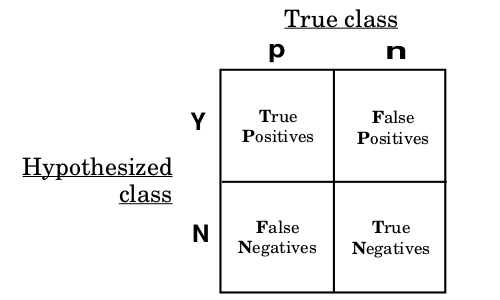
\includegraphics[width=0.8\textwidth]{confusion_matrix.png}
\caption{The confusion matrix}
\label{fig:confusion}
\end{figure}

When reporting the results of a confusible module, the names of the various cells will be replaced by numbers. These numbers are the data needed to calculate various evaluation measures, like the three below. Beside these evaluation measures, I will always give the confusion matrix itself, so readers can calculate other measures if desired.

\item Detection accuracy. Detection accuracy only indicates how many mistakes the confusible detector makes, not what kind of mistakes. It can be calculated with the following formula:

\[
\frac{tp+tn}{tp+tn+fp+fn}
\]

It is similar to prediction accuracy in that it indicates how well the sytem does in general, but keep in mind that prediction and detection accuracy measure two completely different concepts. Although a system with a good prediction accuracy is very likely to also have a good detection accuracy, it might be possible that a system very good at predicting confusibles in errorless texts behaves differently in texts that do contain errors.
 
\item Detection recall and detection precision. 
Precision and recall are concepts well-known within the field of Information Retrieval; precision reflects how much of the retrieved things were relevant, while recall reflects how much of the the relevant things were retrieved. Often there is a inverse relationship between precision and recall: if you change an algorithm so that its recall increases, its precision decreases, and the other way around. In case of spelling checkers, this means you either have a system that catches a lot of errors, but also has a lot of false alarms, or a system that only finds true errors, but also misses a lot; you can't have the best of both.

\[
\frac{tp}{tp+fn}
\]

\[
\frac{tp}{tp+fp}
\]

\item Detection F-score. 
Although you mostly cannot have an optimal precision \emph{and} recall at the same time, you can of course try to have them both as high as possible. Calculating the mean does not help here, because the mean can be relatively high if one of the two is high, but what you want to know is whether \emph{both} are high.

\[
2 * \frac{precision * recall}{precision + recall}
\]

\end{itemize}

\paragraph{Error correction}

\begin{itemize}
\item Confusion matrix.
\item Correction accuracy.
\item Correction recall and correction precision.
\item Correction F-score.
\end{itemize}

\paragraph{Problems with precision and recall.} Some text.

Waarom geen AUC?

\subsection{Results}

\subsection{Conclusion}

\section{General conclusion}

\begin{thebibliography}{99}

\bibitem[Agirre et al., 1998]{agirre98}
Agirre et al., 1998
\bibitem[Brill \& Moore, 2000]{bm00}
Brill \& Moore, 1998
\bibitem[Van Delden et al., 2004]{vandelden04}
Van Delden et al, 2004.
\bibitem[Fawcett, 2004]{fawcett04}
Fawcett, 2004.
\bibitem[Pollock \& Zamora, 1984]{pz84}
Pollock \& Zamora, 1984
\bibitem[Reynaert, 2008]{reynaert08}
Reyneart, 2008.
\bibitem[Starlander \& Popescu-Belis, 2002]{sp02}
Starlander \& Popescu-Belis, 2002
\bibitem[Toutanova \& Moore, 2002]{tm02}
Toutanova \& Moore, 2002.

\end{thebibliography}

% Ene paper Antal

\end{document}
